\pdfminorversion=4
\documentclass[aspectratio=169]{beamer}

\mode<presentation>
{
  \usetheme{default}
  \usecolortheme{default}
  \usefonttheme{default}
  \setbeamertemplate{navigation symbols}{}
  \setbeamertemplate{caption}[numbered]
  \setbeamertemplate{footline}[frame number]  % or "page number"
  \setbeamercolor{frametitle}{fg=white}
  \setbeamercolor{footline}{fg=black}
} 

\usepackage[english]{babel}
\usepackage{inputenc}
\usepackage{tikz}
\usepackage{courier}
\usepackage{array}
\usepackage{bold-extra}
\usepackage{minted}
\usepackage[thicklines]{cancel}
\usepackage{fancyvrb}

\xdefinecolor{ucred}{rgb}{0.50,0,0}
\xdefinecolor{dianablue}{rgb}{0.18,0.24,0.31}
\xdefinecolor{darkblue}{rgb}{0.1,0.1,0.7}
\xdefinecolor{darkgreen}{rgb}{0,0.5,0}
\xdefinecolor{darkgrey}{rgb}{0.35,0.35,0.35}
\xdefinecolor{darkorange}{rgb}{0.8,0.5,0}
\xdefinecolor{darkred}{rgb}{0.7,0,0}
\definecolor{darkgreen}{rgb}{0,0.6,0}
\definecolor{mauve}{rgb}{0.58,0,0.82}

\title[2025-09-11-jupyter-for-teaching]{\textcolor{black}{Jupyter for Teaching}}
\author{Jim Pivarski}
\institute{University of Chicago -- Data Science Institute}
\date{September 11, 2025}

\usetikzlibrary{shapes.callouts}

\begin{document}

\logo{\pgfputat{\pgfxy(0.11, 7.4)}{\pgfbox[right,base]{\tikz{\filldraw[fill=ucred, draw=none] (0 cm, 0 cm) rectangle (50 cm, 1 cm);}\mbox{\hspace{-8 cm}
\includegraphics[height=1 cm]{uchicago-logo-long.png}\hspace{0.1 cm}{
\includegraphics[height=1 cm]{dsi-logo-long.png}}\hspace{0.1 cm}}}}}

\begin{frame}
  \titlepage
\end{frame}

\logo{\pgfputat{\pgfxy(0.11, 7.4)}{\pgfbox[right,base]{\tikz{\filldraw[fill=ucred, draw=none] (0 cm, 0 cm) rectangle (50 cm, 1 cm);}\mbox{\hspace{-8 cm}
\includegraphics[height=1 cm]{uchicago-logo.png}{
\includegraphics[height=1 cm]{dsi-logo.png}}\hspace{0.1 cm}}}}}

% Uncomment these lines for an automatically generated outline.
%\begin{frame}{Outline}
%  \tableofcontents
%\end{frame}

% START START START START START START START START START START START START START

\begin{frame}{Big picture}
\Large
\vspace{0.5 cm}

I almost called this talk ``Literate Programming for Teaching,'' \\ since that's the paradigm.

\vspace{1 cm}
\uncover<2->{Jupyter is just the technology.}
\end{frame}

\begin{frame}{Behold, the ``Tioga'' workstation environment from 1982}
\vspace{0.2 cm}
\begin{columns}
\column{0.95\linewidth}
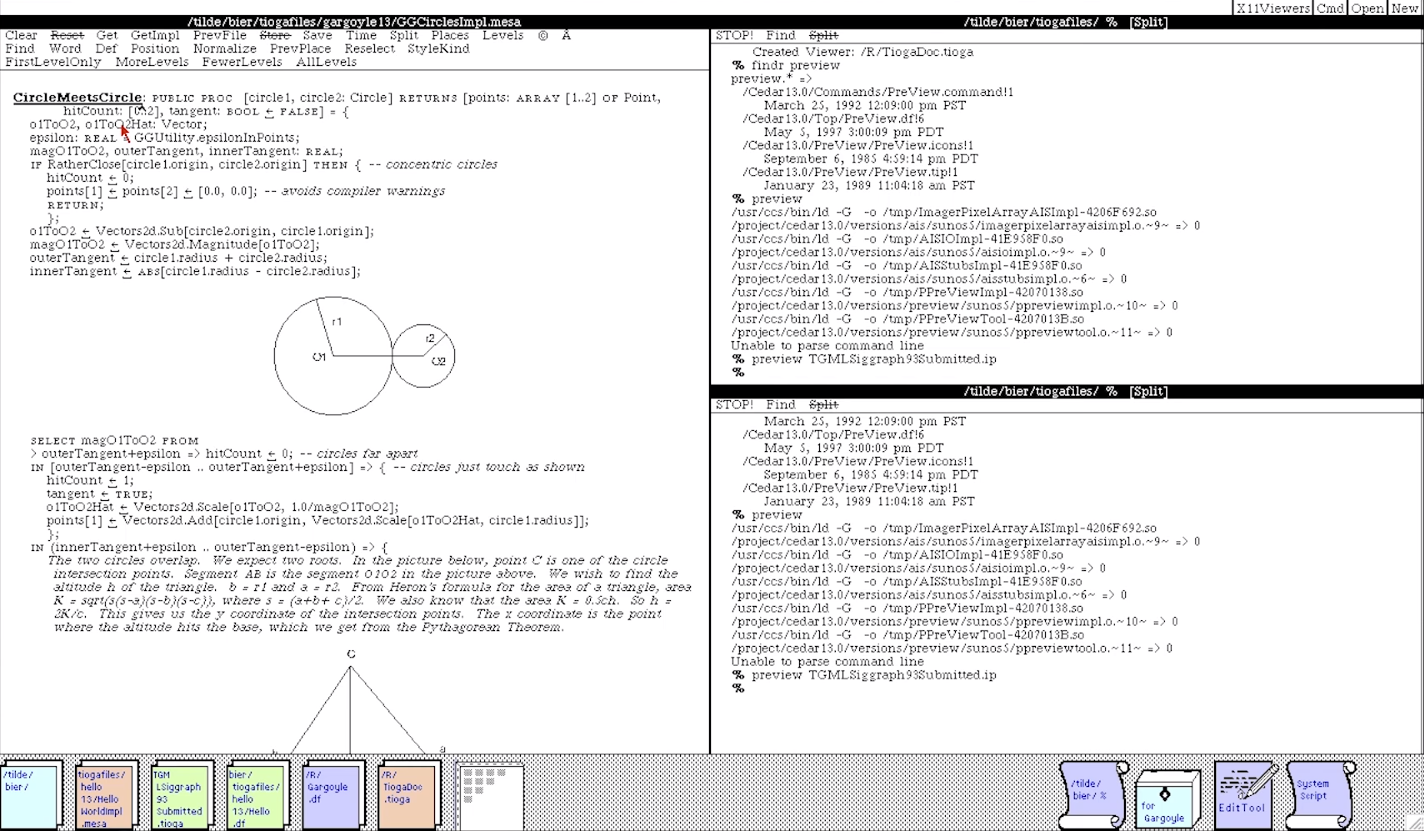
\includegraphics[width=\linewidth]{../img/screenshot-1982-cedar-tioga.png}
\end{columns}
\end{frame}

\begin{frame}{Or ``MathCad'' for personal computers in 1986}
\vspace{0.2 cm}
\begin{columns}
\column{0.73\linewidth}
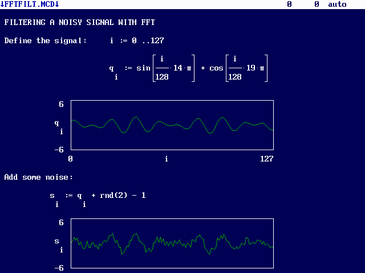
\includegraphics[width=\linewidth]{../img/screenshot-1986-mathcad.png}
\end{columns}
\end{frame}

\begin{frame}{``Mathematica'' in 1987 was the first of these to be mainstream}
\vspace{0.2 cm}
\begin{columns}
\column{0.83\linewidth}
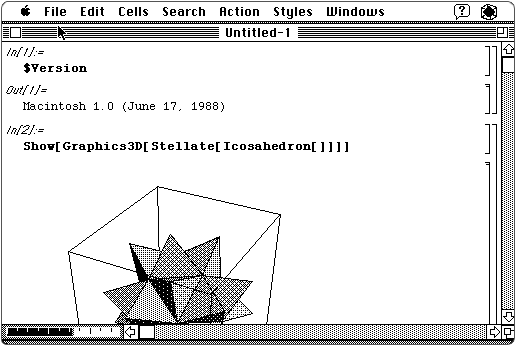
\includegraphics[width=\linewidth]{../img/screenshot-1987-mathematica.png}
\end{columns}
\end{frame}

\begin{frame}{Jupyter wasn't even the first to use web browsers and Python}
\vspace{0.2 cm}
\begin{columns}
\column{0.54\linewidth}
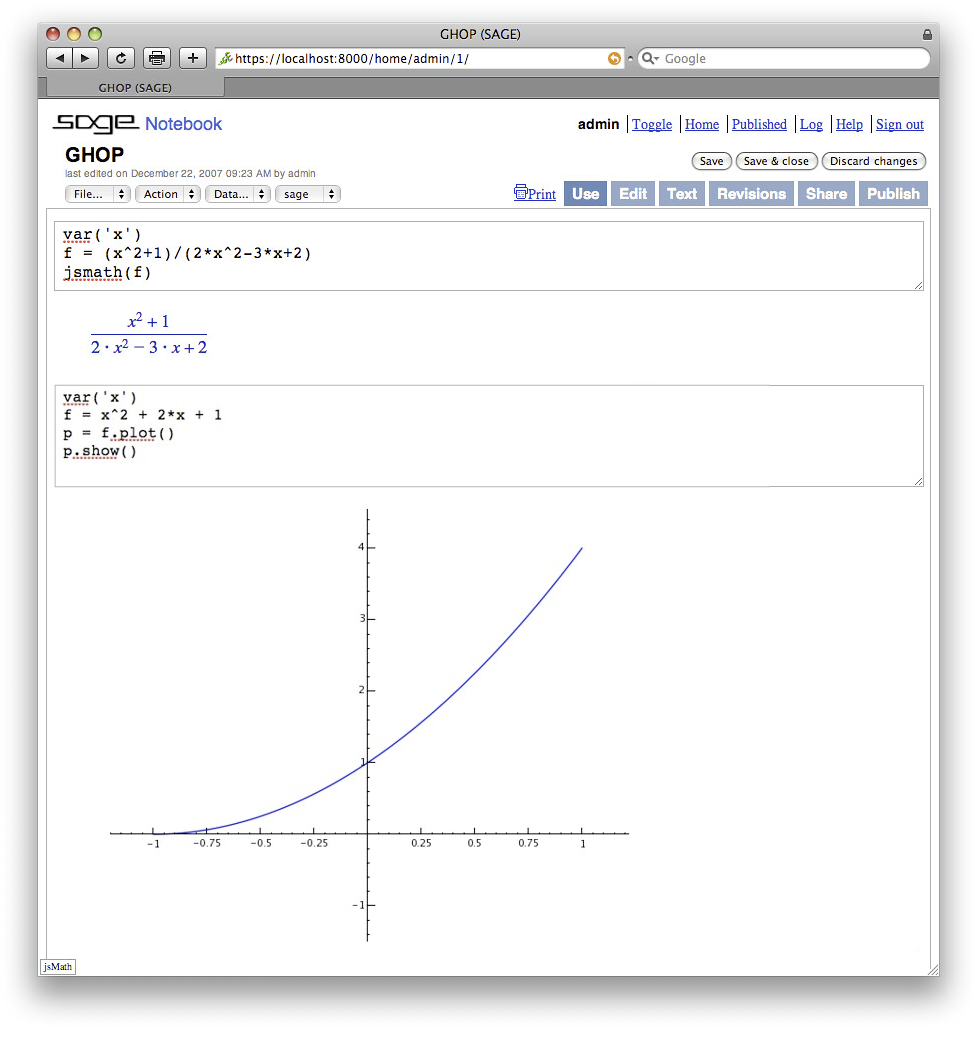
\includegraphics[width=\linewidth]{../img/screenshot-2007-sage.png}

\column{0.5\linewidth}
\Large
This is ``SAGE'' in 2007.
\end{columns}
\end{frame}

\begin{frame}{Jupyter started life as ``IP[y]: Notebook'' in 2012}
\vspace{0.2 cm}
\begin{columns}
\column{0.6\linewidth}
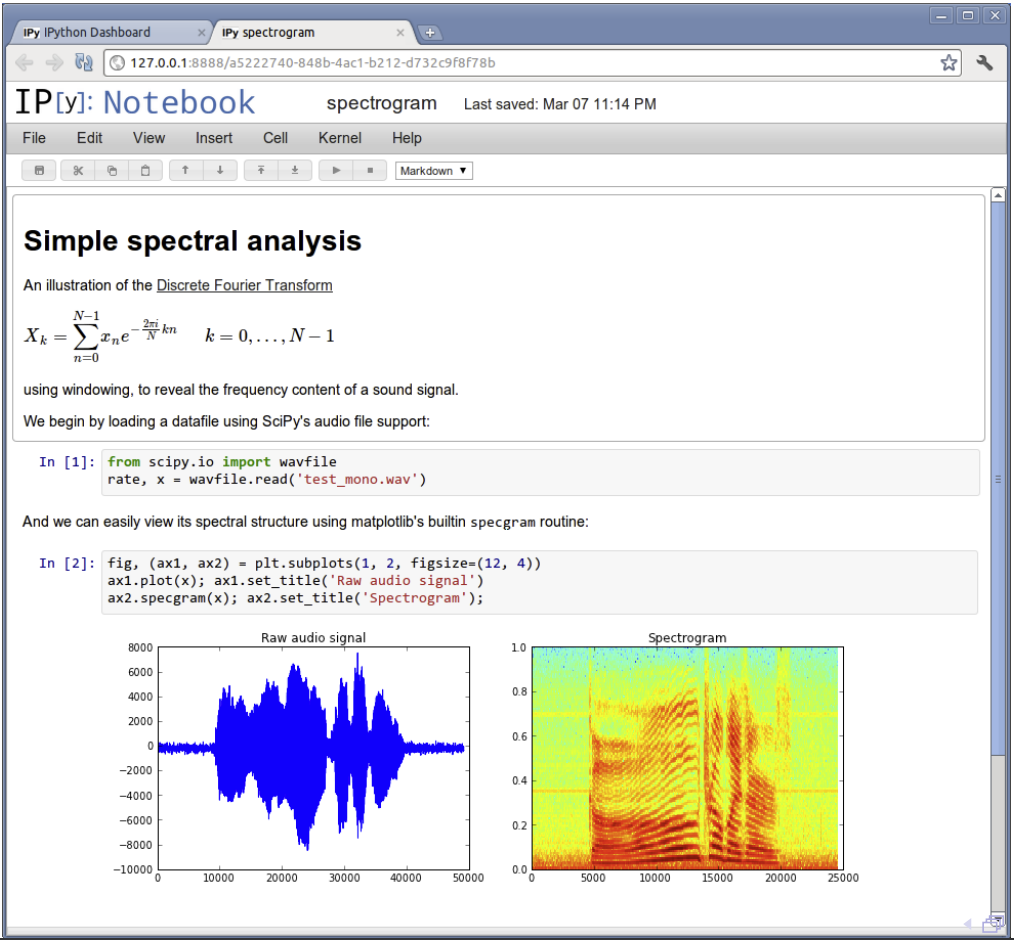
\includegraphics[width=\linewidth]{../img/screenshot-2012-ipython-notebook.png}
\end{columns}
\end{frame}

\begin{frame}{But changed its name in 2015 to say it's for \textcolor{yellow}{\bf Ju}lia, \textcolor{yellow}{\bf Pyt}hon, and \textcolor{yellow}{\bf R}}
\vspace{0.2 cm}
\begin{columns}
\column{0.52\linewidth}
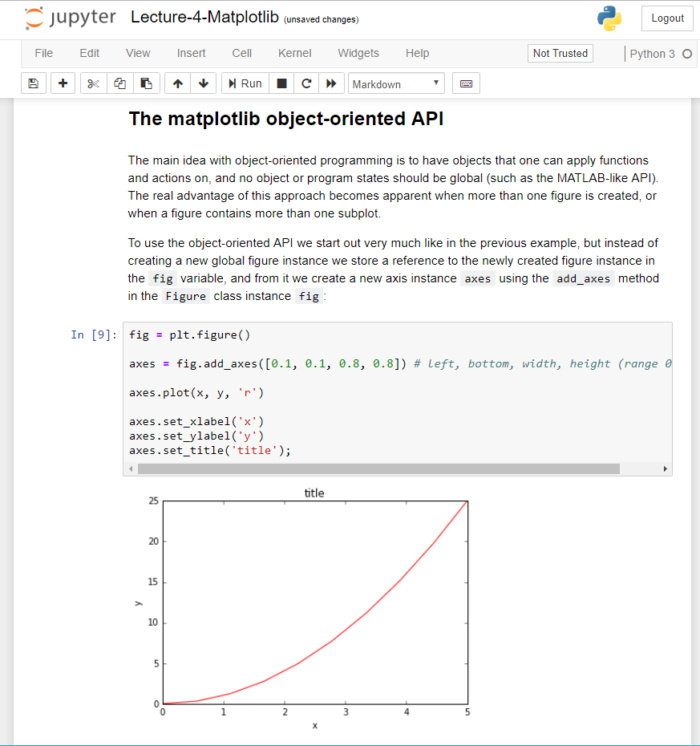
\includegraphics[width=\linewidth]{../img/screenshot-2015-jupyter-notebook.png}

\column{0.5\linewidth}
\Large
\textcolor{gray}{(However, Julia programmers more often use Pluto.jl and R programmers often use RStudio.)}
\end{columns}
\end{frame}

\begin{frame}{Notebooks are the middle of 3 fundamental modes of programming}
\vspace{0.2 cm}
\begin{columns}
\column{\linewidth}
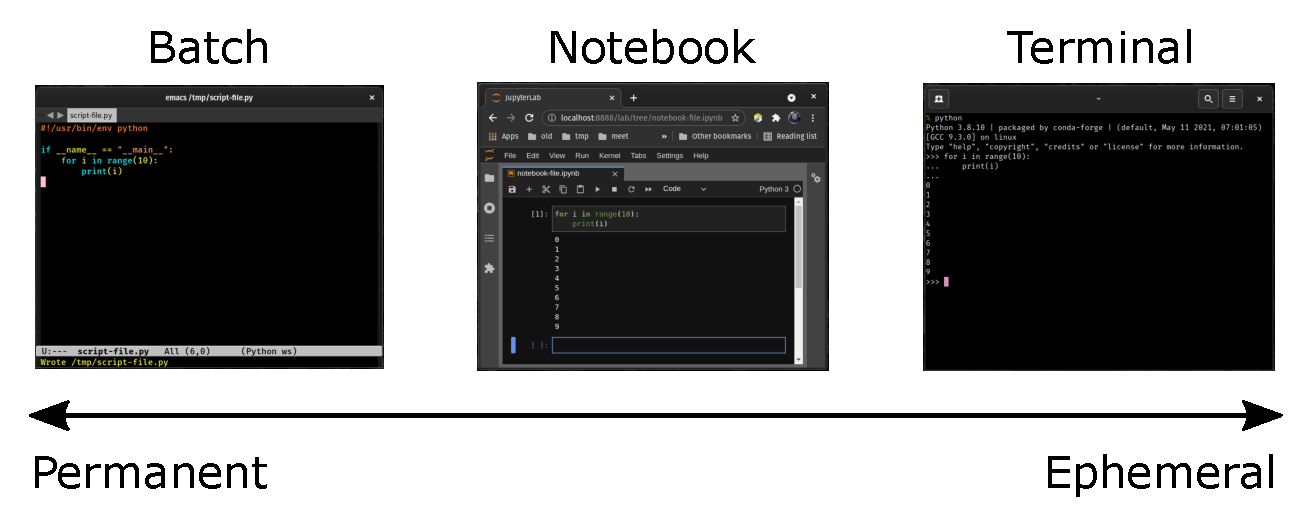
\includegraphics[width=\linewidth]{../img/fundamental-3-modes-of-programming.pdf}
\end{columns}
\end{frame}

\begin{frame}{Batch: the most permanent}
\vspace{0.2 cm}
\begin{columns}
\column{0.45\linewidth}
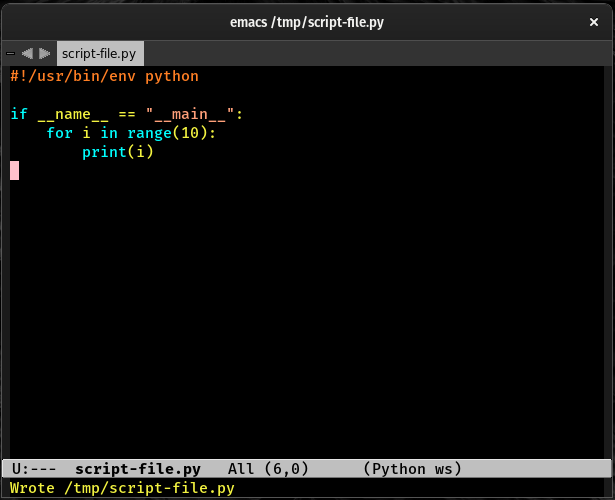
\includegraphics[width=\linewidth]{../img/fundamental-3-modes-batch.png}

\column{0.5\linewidth}
\large
\begin{itemize}\setlength{\itemsep}{0.25 cm}
\item<1-> This is the oldest, from the punch-card, time-scheduling era.
\item<2-> Best for developing software libraries, with an emphasis on architecture and the large scale.
\item<3-> Testing means running the whole program from scratch (maybe even compiling it if you're using one of {\it those} languages).
\item<4-> Conceit: you're a sculptor, carving a beautiful ediface that will stand the test of time.
\end{itemize}
\end{columns}
\end{frame}

\begin{frame}{Terminal: the most ephemeral}
\vspace{0.2 cm}
\begin{columns}
\column{0.45\linewidth}
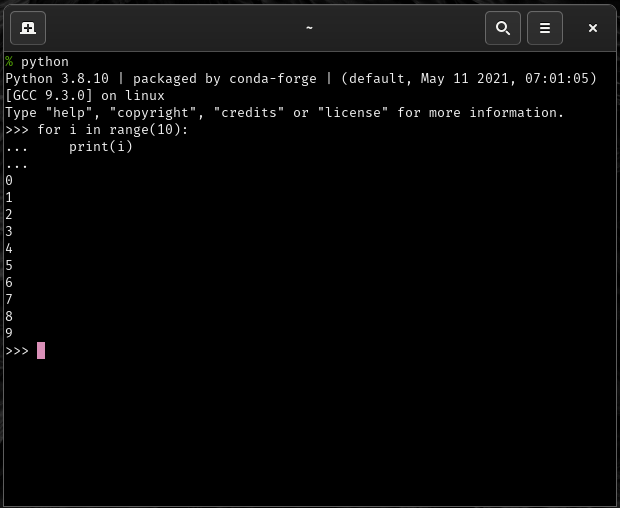
\includegraphics[width=\linewidth]{../img/fundamental-3-modes-terminal.png}

\column{0.53\linewidth}
\large
\begin{itemize}\setlength{\itemsep}{0.25 cm}
\item<1-> Also has a long history in interactive languages like LISP, SPEAKEASY, and BASIC, as well as filesysstem shells like UNIX and VAX.
\item<2-> Best for getting quick answers like, ``What are the first few elements of this list?'' or making simple changes like, ``Convert all the images in this directory to JPEG.''
\item<3-> Testing is continuous and immediate.
\item<4-> Conceit: you're a hack3r, mashing out commands at a breakneck pace.
\end{itemize}
\end{columns}
\end{frame}

\begin{frame}{Notebook: in between}
\vspace{0.2 cm}
\begin{columns}
\column{0.45\linewidth}
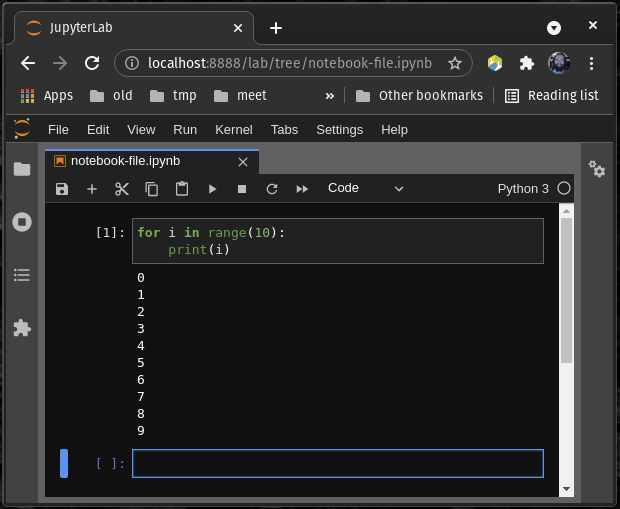
\includegraphics[width=\linewidth]{../img/fundamental-3-modes-notebook.png}

\column{0.53\linewidth}
\large
\begin{itemize}\setlength{\itemsep}{0.25 cm}
\item<1-> Perceived as new, but it's had an important place in mathematical and data analysis software for almost as long as the spreadsheet (1979).
\item<2-> Best for quick analyses that will likely be repeated: iterative investigation. Or for presenting code with detailed explanations, like a book, or teaching and running code in real-time.
\item<3-> Conceit: Literate Programming!
\end{itemize}
\end{columns}
\end{frame}









\end{document}
